%\documentclass{report}
%\usepackage{sectsty}
%%\usepackage{minitoc} % for contents 
%\chapterfont{\raggedleft}

%\begin{document}
%\dominitoc[n]
%\nomtcpagenumbers



\chapter{Background \& Technical Information}
	\minitoc
	%\addtocontents{toc}{\protect\contentsline{chapter}{\protect\numberline{}Background \& Technical Information}{}{}}
	\section{Base ISA Overview}
	\label{sec:Overview}
	The RISC-V ISA is defined as a base integer ISA, which must be present in any implementation, plus optional extensions to the base ISA. The base integer ISA is very similar to that of the early RISC processors except with no branch delay slots and with support for optional variable-length instruction encodings. \\
	
	The base integer ISA is named "I" (prefixed by RV32 or RV64 depending on integer register width) and contains integer computational instructions, integer loads, integer stores and control-flow instructions and is mandatory for all RISC-V implementations.
	\clearpage
	\section{ISA Extensions}
	\label{sec:Extensions}
	There are various extensions to the Base ISA ("I") such as:  \\\\
	\vspace{-2mm}
	\begin{tabular}{|c|l|} \hline
	\setrow{\bfseries}Extension Symbol &\setrow{\bfseries} Extension Contents \\\hline
		%%%%%%%%%%%%%%%%%%%%%%%%%%%%%%%%%%%%%%%%%%%%%%%%%%%%%
		"M" & Integer Multiplication \& Division     \\\hline
		"A" & Atomic Instructions 				     \\\hline
		"F" & Single-Precision Floating Point		 \\\hline
		"D" & Double-Precision Floating Point 		 \\\hline
		"Q" & Quad-Precision Floating Point          \\\hline
		"L" & Decimal Floating Point                 \\\hline
		"C" & Compressed Instructions                \\\hline
		"B" & Bit Manipulation 					     \\\hline
		"J" & Dynamically Translated Languages 		 \\\hline
		"T" & Transactional Memory 					 \\\hline
		"P" & Packed SIMD Instructions 			     \\\hline
		"V" & Vector Operations 					 \\\hline
		"N" & User-Level Interrupts					 \\\hline
	\end{tabular}
	\captionof{table}{"ISA Extensions"} 
	\vspace{5mm}
	\par
	Therefore, various architectures can come up as a mix of some of those extensions. For example an integer base ISA plus the extensions "M","A","F","D" is given the abbreviation "G" and provides a general-purpose scalar instruction set. The $RV32G$ and $RV64G$ are the considered to be the default architectures.
	
	\section{The RV32I}
	\label{sec:RV32I}
	\subsection{Instruction Length Encoding}
	\label{subsec:ILE}
	The base RISC-V ISA (RV32I) has fixed-length 32-bit instructions that must be naturally aligned on 32-bit boundaries. All the 32-bit instructions in this ISA have their lowest two bits set to $11$.
	\vspace{3mm}
	\begin{figure}[h!]
		
		\begin{center}
		
\includegraphics[width=0.6\textwidth]{InstructionLengthEncoding}
		\caption{RV32I Instruction Length Encoding}
		\label{image2.1}
		\end{center}
	\end{figure}
	\subsection{Base ISA Model}
	\label{subsec:ISA Model}
	There are 31 general-purpose registers x1-x32, which hold integer values. Register x0 is hardwired to the constant 0. There is one additional user-visible register: the program counter \textbf{pc} holds the address of the current instruction.
	\subsection{Instruction and Immediate Formats} \label{sect2.3.3}
	There are four core instruction formats (R/I/S/U). All are fixed 32 bits in length and must be        aligned on a four-byte boundary in memory. There are a further two variants of the instruction formats (B/J) based on the handling of immediates.\\
	\begin{figure}[h!]
		
		\begin{center}
			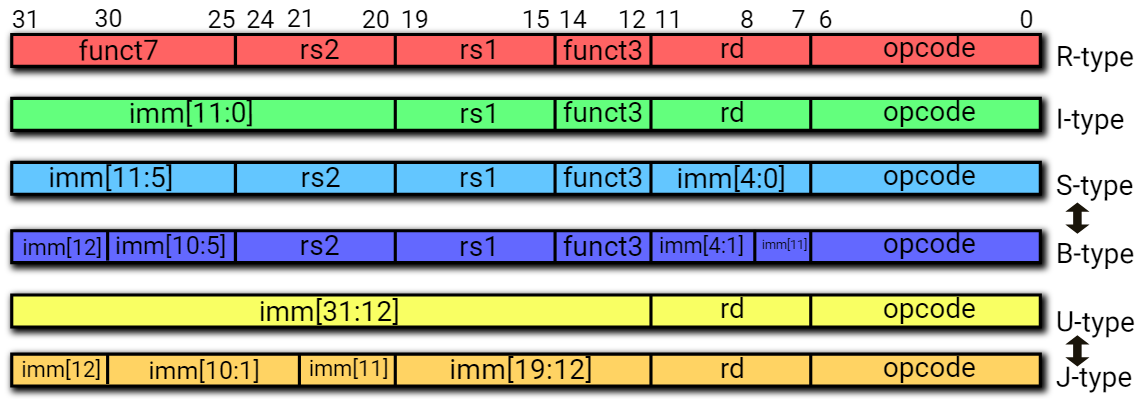
\includegraphics[width=1\textwidth]{CommandTypes}
			\caption{Instruction Types}
			\label{Image2.2}
		\end{center}
	\end{figure}
	\\

	The only difference between the S and B formats is that the 12-bit immediate field is used to encode branch offsets in multiples of 2 in the B format. Instead of shifting all bits in the instruction-encoded immediate left by one in hardware as is conventionally done, the middle bits (imm[10:1]) and sign bit stay in fixed positions, while the lowest bit in S format (inst[7]) encodes a high-order bit in B format.
	\\
	
	Similarly, the only difference between the U and J formats is that the 20-bit immediate is shifted left by 12 bits to form U immediates and by 1 bit to form J immediates. The location of instruction bits in the U and J format immediates is chosen to maximize overlap with the other formats and with each other.\\
	
	\begin{figure}[h!]
		
		\begin{center}
			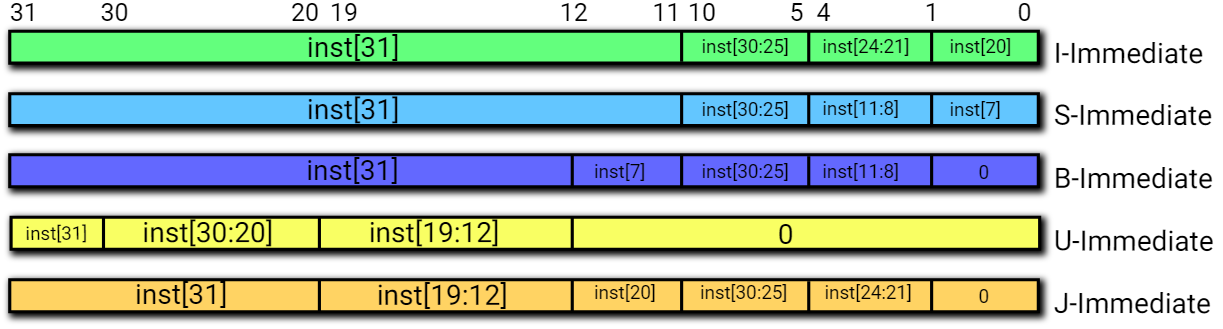
\includegraphics[width=1\textwidth]{ImmediateTypes}
			\caption{Immediate Types}
			\label{Image2.3}
		\end{center}
	\end{figure}

	The fields of Figure \ref{Image2.3} are labeled with the instruction bits (instr[y]) used to construct their value. Sign extension always uses inst[31]. \\
	
	Labeled as $rd$ is the destination register, meaning the register at which the result of the operation will be stored and as $rs1,rs2$ (if any) are the registers (operands) that will be used. The $funct7,funct3$ and $opcode$ fields will be used for the decode of the command and for the generation of the signals needed for its processing while the $imm[x:y]$ fields will be used for the assemble of the command's immediate.	
	\newpage
	\subsection{The Instructions}
	\label{subsec:ActualInstructions}
	\subsubsection{Integer Computational Instructions}
	\label{subsubsec:IntegerInstr}
	Most integer computational instructions operate on XLEN (= 32) bits of values held in the integer register file. Integer computational instructions are either encoded as register-immediate operations using the I-type format or as register-register operations using the R-type format. The destination is register $rd$ for both register-immediate and register-register instructions. \\
	Note that there is not a special instruction set support for overflow checks on integer arithmetic operations in the RV32I ISA. Overflow checks can be cheaply implemented using branches. \\
	The commands on the tables below follow the color-code of  Figure~\ref{Image2.2} and Figure~\ref{Image2.3} \\
	\vspace{4mm}
	\textbf{ {\footnotesize[A] Integer Register-Immediate Instructions }} \\
	
	\begin{threeparttable}
		\begin{tabular}{|c|p{3in}|p{1in}|} \hline
		\setrow{\bfseries}Command &\setrow{\bfseries} Operation &\setrow{\bfseries} Syntax 	\\\hline
		\cellcolor{brightgreen}ADDI & {\small Addition between $imm$ and $rs1$} & {\small $addi$ $rd,rs1,imm$} 	\\\hline
		\cellcolor{brightgreen}SLTI & {\small If $rs1<imm$ then $rd\leftarrow1$ else $rd\leftarrow0$} & {\small $slti$ $rd,rs1,imm$} \\\hline
		\cellcolor{brightgreen}SLTIU& {\small Same as SLTI, but UNSIGNED} &{\small $sltiu$ $rd,rs1,imm$} 			\\\hline
		\cellcolor{brightgreen}ANDI & {\small Bitwise AND between $rs1$ and $imm$} & {\small $andi$ $rd,rs1,imm$}	\\\hline
		\cellcolor{brightgreen}ORI  & {\small Bitwise OR between $rs1$ and $imm$} & {\small $ori$ $rd,rs1,imm$}   \\\hline
		\cellcolor{brightgreen}XORI & {\small Bitwise XOR between $rs1$ and $imm$} & {\small $xori$ $rd,rs1,imm$} \\\hline
		\cellcolor{brightgreen}SLLI & {\small Shift left logical of $rs1$ by given shift amount ($imm$)} & {\small $slli$ $rd,rs1,imm$} \\\hline
		\cellcolor{brightgreen}SRLI & {\small Shift right logical of $rs1$ by given shift amount($imm$)} &
		{\small $srli$ $rd,rs1,imm$} \\\hline
		\cellcolor{brightgreen}SRAI & {\footnotesize Shift right arithmetic of $rs1$ by given shift amount($imm$)} &
		{\small $srai$ $rd,rs1,imm$} \\\hline
		\cellcolor{canaryyellow}LUI &{\small $rd\leftarrow imm$} & {\small $lui$ $rd,imm$} \\\hline
		\cellcolor{canaryyellow}AUIPC&{\small $rd\leftarrow pc+imm$} & {\small $auipc$ $rd, imm$} \\\hline
			
		\end{tabular}

		 \begin{tablenotes}
		 	
			\footnotesize
			\item Notes:
			\item
			 \underline{\textbf{\textcolor{brightgreen}{$\rightarrow$}}} The arithmetic operations that include addition \underline{ignore} overflow scenarios as mentioned before. The immediates used in those commands are I-type Immediates and they are generated as shown at Figure~\ref{Image2.3}. Shifts by a constant are encoded as a specialization of the I-type format. The operand to be shifted is in $rs1$, and the shift amount is encoded in the lower 5 bits of the I-immediate field.
			\item 
			\underline{\textbf{\textcolor{canaryyellow}{$\rightarrow$}}} Those two instructions are of the U-type and use the respective Immediate types as well.  LUI stands for "Load Upper Immediate" while AUIPC stands for "Add Upper Immediate To PC". Again one can recur at Figure~\ref{Image2.3} for further details on the subject of Immediate generation.
			\captionof{table}{Register-Immediate Instructions}
			\label{subsubsec:table2.2}
			\vspace{4cm}
		\end{tablenotes}
	\end{threeparttable}
	
	\textbf{ {\footnotesize[B] Integer Register-Register Instructions }} \\
	
	\begin{threeparttable}
		\begin{tabular}{|c|p{3in}|p{1in}|} \hline
			\setrow{\bfseries}Command &\setrow{\bfseries} Operation &\setrow{\bfseries} Syntax 	\\\hline
			\cellcolor{bred}ADD & {\small Addition between $rs1$ and $rs2$} & {\small $add$ $rd,rs1,rs2$} 	\\\hline
			\cellcolor{bred}SUB & {\small Subtraction between $rs1$ and $rs2$} & {\small $sub$ $rd,rs1,rs2$}  \\\hline
			\cellcolor{bred}SLT & {\small If $rs1<rs2$ then $rd\leftarrow1$ else $rd\leftarrow0$} & {\small $slt$ $rd,rs1,rs2$} \\\hline
			\cellcolor{bred}SLTU & {\small Same as SLT, but UNSIGNED} &{\small $sltu$ $rd,rs1,rs2$} 			\\\hline
			\cellcolor{bred}AND  & {\small Bitwise AND between $rs1$ and $rs2$} & {\small $and$ $rd,rs1,rs2$} \\\hline
			\cellcolor{bred}OR   & {\small Bitwise OR between $rs1$ and $rs2$}  & {\small $or$ $rd,rs1,rs2$}  \\\hline
			\cellcolor{bred}XOR  & {\small Bitwise XOR between $rs1$ and $rs2$} & {\small $xor$ $rd,rs1,rs2$} \\\hline
			\cellcolor{bred} SLL & {\small Shift left logical of $rs1$ by given shift amount ($rs2$)}& {\small $sll$ $rd,rs1,rs2$} \\\hline
			\cellcolor{bred} SRL & {\small Shift right logical of $rs1$ by given shift amount ($rs2$)} & {\small $srl$ $rd,rs1,rs2$} \\\hline
			\cellcolor{bred} SRA & {\footnotesize Shift right arithmetic of $rs1$ by given shift amount ($rs2$)} & {\small $sra$ $rd,rs1,rs2$} \\\hline
			
		\end{tabular}
	
		 \begin{tablenotes}
			
			\footnotesize
			\item Notes:
			\item
			The shift amount is now held in the lower 5 bits of register $rs2$.
			\captionof{table}{Register-Register Instructions}
			\label{subsubsec:table2.3}
			\vspace{5mm}
		\end{tablenotes}

	\end{threeparttable}
	
	\textbf{ {\footnotesize[C] NOP Instruction }} \\
	
	The NOP instruction does not change any user-visible state, except for advancing the \textbf{pc}. NOP is encoded as $ADDI$ $x0,x0,0$. 
	\vspace{5mm}
	
	\subsubsection{Control Transfer Instructions}
	\label{subsubsec:ControlTransferInstr}
	
	The RV32I ISA provides two types of control transfer instructions: unconditional jumps and conditional branches. Control transfer instructions in RV32I do not have architecturally visible delay slots.\\
	
	\textbf{ {\footnotesize[A] Unconditional Jumps }} \\
	
	\begin{threeparttable}
		\begin{tabular}{|c|p{3in}|p{1in}|} \hline
			\setrow{\bfseries}Command &\setrow{\bfseries} Operation &\setrow{\bfseries} Syntax 	\\\hline
			\cellcolor{carorange}JAL & {\footnotesize $GOTO$ $pc+imm$ and $rd\leftarrow pc+4$} & $jal$ $rd,imm$ \\\hline
			\cellcolor{brightgreen}JALR & {\footnotesize $GOTO$ $(rs1+imm)[31:1]\&0$ and $rd\leftarrow pc+4$} & {\small$jalr$ $rd,rs1,imm$}\\\hline 
		\end{tabular}
		\begin{tablenotes}
		\footnotesize	
		\item 
		Notes:
		\item 
		\underline{\textbf{\textcolor{carorange}{$\rightarrow$}}} JAL (Jump and Link) is a J-type instruction. J-immediate encodes a signed offset in multiples of 2 bytes. The offset is sign-extended and added to the pc, to form the jump target address. Jumps can therefore target a $\pm1MiB range$. JAL stores the address of the instruction following the jump (pc+4) into register rd.
		\item 
		\underline{\textbf{\textcolor{brightgreen}{$\rightarrow$}}} JALR (Jump and Link Register) uses the I-type encoding. The jump target address is obtained by adding the 12-bit signed I-immediate to the register rs1, then setting the least-significant bit of the result to zero. The address of the instruction following the jump (pc+4) is written to register rd.
		\end{tablenotes}
		\captionof{table}{Uncoditional Jumps}
		\label{subsubsec:table2.4}
		\vspace{1cm}
	\end{threeparttable}

	\textbf{ {\footnotesize[B] Conditional Branches }} \\
	
	All branch instructions use the B-type instruction format. The 12-bit B-immediate encodes signed offsets in multiples of 2 and is added to the current pc to give the target address. The conditional branch range is $\pm4KiB$.\\
	
	\begin{threeparttable}
	
		\begin{tabular}{|c|p{3in}|p{1in}|} \hline
		\setrow{\bfseries}Command &\setrow{\bfseries} Operation &\setrow{\bfseries} Syntax 					 \\\hline
		\cellcolor{blue} BEQ & {\small $if$ $rs1=rs2$ then $JUMP$} & {\small $beq$ $rs1,rs2,imm$} 		 \\\hline
		\cellcolor{blue} BNE & {\small $if$ $rs1\neq rs2$ then $JUMP$} & {\small $bne$ $rs1,rs2,imm$} 	 \\\hline
		\cellcolor{blue} BLT & {\small $if$ $rs1<rs2$ then $JUMP$} & {\small $blt$ $rs1,rs2,imm$}		 \\\hline 
		\cellcolor{blue} BLTU & {\small Same as BLT, but UNSIGNED } & {\small $bltu$ $rs1,rs2,imm$}		 \\\hline
		\cellcolor{blue} BGE  & {\small $if$ $rs1\geq rs2$ then $JUMP$} & {\small $bge$ $rs1,rs2,imm$} 	 \\\hline
		\cellcolor{blue} BGEU & {\small Same as BGE, but UNSIGNED } & {\footnotesize $bgeu$ $rs1,rs2,imm$}\\\hline
		\end{tabular}
		
		\begin{tablenotes}
			\footnotesize
			\item 
			Notes:
			\item 
			The commands BGT, BGTU, BLE and BLEU can be synthesized by reversing the operands to BLT, BLTU, BGE and BGEU respectively.
			\captionof{table}{Conditional Branches}
			\label{subsubsec:table2.5}
			\vspace{5mm}
		\end{tablenotes}
		
	\end{threeparttable}
	
	\subsubsection{Load and Store Instructions}
	\label{subsubsec:LoadsStores}		
	
	
	RV32I is a load-store architecture, where only load and store instructions access memory and arithmetic instructions only operate on CPU registers. RV32I provides a 32-bit user address space that is byte-addressed and little-endian.
	The effective address in both cases is obtained by adding register $rs1$ to the sign-extended 12-bit offset.\vspace{3mm}
	
		\begin{threeparttable}
		
		\begin{tabular}{|c|p{3in}|p{1in}|} \hline
			
			\setrow{\bfseries}Command &\setrow{\bfseries} Operation &\setrow{\bfseries} Syntax 					 		 \\\hline
			\cellcolor{brightgreen} LW & {\small $rd\leftarrow MEM[31:0]$} & {\small $lw$ $rd,imm(rs1)$}		         \\\hline
			\cellcolor{brightgreen} LH & {\small $rd\leftarrow MEM[31:16]$ or $MEM[15:0]$} & {\small $lh$ $rd,imm(rs1)$} \\\hline
			\cellcolor{brightgreen} LHU &{\small Same as LH, but UNSIGNED} & {\small $lhu$ $rd,imm(rs1)$}                \\\hline
			\cellcolor{brightgreen} LB & {\footnotesize $rd\leftarrow MEM[31:24]$ or $MEM[23:16]$ or $MEM[15:8]$ or $MEM[7:0]$}
			& {\small $lb$ $rd,imm(rs1)$}                                                                                \\\hline
			\cellcolor{brightgreen} LBU &{\small Same as LB, but UNSIGNED} & {\small $lbu$ $rd,imm(rs1)$}                \\\hline
			\cellcolor{capri!75} SW & {\small $MEM\leftarrow rs2$} & {\small $sw$ $rs2,imm(rs1)$}                        \\\hline
			\cellcolor{capri!75} SH & {\small $MEM[31:16]$ or $MEM[15:0]$ $\leftarrow rs2[15:0]$} &{\small $sh$ $rs2,imm(rs1)$}                                                                                              \\\hline
			\cellcolor{capri!75} SB & {\footnotesize $MEM[31:24]$ or $MEM[23:16]$ or $MEM[15:8]$ or $MEM[7:0]$ $\leftarrow rs2[7:0]$}
			& {\small $sb$ $rs2,imm(rs1)$}                                                                               \\\hline
			
		\end{tabular}
		
		\begin{tablenotes}
			
			\footnotesize
			\item 
			Notes:
			\item 
			The choosing of the byte that will be written or loaded in any case is done by the 2 least-significant bits of the calculated effective address.
			\item
			\underline{\textbf{\textcolor{brightgreen}{$\rightarrow$}}} In case of LH/LB operations, the loaded value will be sign-extended up to 32-bits while in case of LHU/LBU, the value will be zero-filled up to 32-bits.
			\item 
			\underline{\textbf{\textcolor{capri!75}{$\rightarrow$}}} Always the least-significant bits of the register $rs2$ are being stored at SH and SB operations.
			
		\end{tablenotes}
	
		\captionof{table}{Loads and Stores}
		\label{subsubsec:table2.6}
		\vspace{5mm}
		
	\end{threeparttable}

	
	
%\end{document}